\documentclass[11pt,a4paper,twocolumn]{article}

% === Core Packages ===
\usepackage[margin=2cm]{geometry}
\usepackage[utf8]{inputenc}
\usepackage[T1]{fontenc}
\usepackage{times}
\usepackage{amsmath,amssymb}
\usepackage{graphicx}
\usepackage{booktabs}
\usepackage{float}
\usepackage{enumitem}
\usepackage{tikz}
\usepackage{pgfplots}
\pgfplotsset{compat=1.18}
\usetikzlibrary{arrows.meta,shapes.geometric,positioning,calc,decorations.markings,fit,backgrounds}

% === Citation (IEEE style) ===
\usepackage[numbers,sort&compress]{natbib}
\bibliographystyle{IEEEtranN}

% === Hyperref ===
\usepackage[hidelinks]{hyperref}
\usepackage{xurl}

% === Settings ===
\setlength{\parindent}{1em}
\setlength{\parskip}{0.3em}

% === PDF metadata ===
\hypersetup{
  pdftitle={Decentraliserat ryktesnätverk: Ett ramverk för naturlig samhällsorganisation},
  pdfauthor={Pavel Kudrna},
  pdfsubject={Personix — a decentralized reputation network},
  pdfkeywords={Personix, decentralized reputation, reputation social network,
    decentralized identifiers, DID, meritocracy, censorship resistance},
}

% === Title ===
\title{\textbf{Decentraliserat ryktesnätverk:\\Ett ramverk för naturlig samhällsorganisation}}
\author{Pavel Kudrna\\Personix Project --- \url{https://personix.org}\\Prague, Czechia\\Draft v1 --- March 2026}
\date{}

\begin{document}
\maketitle

% ============================================================
% ABSTRACT
% ============================================================
\begin{abstract}
Rättskänslan---övertygelsen om att oförrätter rättas till och att förtjänst belönas---är samhällets starkaste sammanhållande kraft. När centraliserade styrningsinstitutioner inte kan leverera denna känsla, eftersom kostnaden för att göra en rättighet gällande överstiger själva rättighetens värde, urholkas den sociala sammanhållningen. Nuvarande institutionella strukturer misslyckas med att lösa en betydande klass av tvister systematiskt på samma sätt som central planering misslyckas med att fördela resurser: genom informationsasymmetri, saknade återkopplingsslingor och avståndet mellan beslutsfattare och konsekvenserna av deras beslut. Denna uppsats presenterar ett ryktes-socialt nätverk (RSN): ett decentraliserat, omutbart, censurresistent kommunikationslager byggt på decentraliserade identifierare (DID) som gör det möjligt för pseudonyma deltagare att publicera, verifiera och konsumera ryktesinformation om beteende i verkligheten. Kärnmekanismen vilar på tre designprinciper: (1)~en asymmetrisk kostnadsstruktur där läsning av ryktesdata är billig men skrivande kräver verifierbar ansträngning; (2)~ett ickedeterministiskt protokoll för val av verifierare baserat på konsekvent hashning som prissätter radikala påståenden genom eskalerande iterationskostnader; och (3)~en marknadsdriven modell för ryktesauktoritet där privata verifierare satsar sitt ackumulerade rykte på riktigheten i de påståenden de stödjer. Den resulterande arkitekturen frambringar en emergent meritokrati utan central samordning och möjliggör en gradvis, reversibel migrationsväg från befintliga statligt administrerade system.
\end{abstract}

% ============================================================
% 1. INTRODUCTION
% ============================================================
\section{Inledning}

\subsection{Problemet med centraliserat förtroende}

Modern styrning vilar på ett grundläggande antagande: att centraliserade institutioner kan förmedla förtroende mellan främlingar i stor skala. Domstolar avgör tvister. Register intygar ägande. Tillsynsorgan upprätthåller standarder. Dessa institutioner utformades i en tid då information var knapp, kommunikation var långsam och delegering av auktoritet till ett centralt organ var den enda genomförbara samordningsmekanismen. Centraliserad styrning misslyckas dock av samma strukturella skäl som central planering: informationsasymmetri, saknade återkopplingsslingor och avståndet mellan beslutsfattare och konsekvenserna av deras beslut.

Antagandet brister till exempel när kostnaden för institutionell förmedling överstiger tvistens värde. Betrakta en hyresgäst som upptäcker att den hyrda lägenheten saknar ett lagstadgat elsäkerhetsintyg---ett förhållande som utgör en omedelbar livsfara. Hyresgästens juridiska rätt att frånträda avtalet är otvetydig. Ändå överstiger kostnaden för att göra denna rätt gällande genom domstolssystemet det penningmässiga värdet av depositionen och det skadestånd som är skyldigt, även med potentiell lagstadgad ersättning inräknad~\cite{czcourtfees}. Det rationella svaret är att bära förlusten och lämna.

Detta är inte ett patologiskt gränsfall. Det är standarderfarenheten för en betydande klass av tvister där skadan är verklig men de penningmässiga insatserna faller under tröskeln där institutionell verkställighet blir ekonomiskt rationell. Resultatet är ett system som strukturellt gynnar illasinnade aktörer: de som skadar andra i volymer under denna tröskel kan agera ostraffat, eftersom kostnaden för att söka rättvisa faller på den skadade parten.

Exemplet ovan är hämtat från författarens juridiska miljö---det tjeckiska civilrättssystemet. I andra rättstraditioner---prejudikatsbaserad sedvanerätt, sedvänjerätt, blandade system---misslyckas rättvisan på olika sätt och i olika grad, beroende på jurisdiktionens kulturella och processuella särdrag. Läsare kommer sannolikt att känna igen motsvarande exempel från sitt eget sammanhang. Det som är strukturellt universellt är mönstret: tvister vars värde faller under tröskeln för ekonomiskt rationell verkställighet slutar med att förlusten bärs av den skadade parten. RSN utlovar inte perfekt rättvisa---det minskar enbart den strukturella fördel som illasinnade aktörer åtnjuter när institutionell verkställighet är olönsam.

\subsection{Varför befintliga lösningar inte räcker till}

\textbf{Ramverk för decentraliserad identitet (DID)}~\cite{did2022} tillhandahåller kryptografiska mekanismer för självsuverän identitetshantering men fokuserar främst på identitetsverifiering utan att ta itu med den bredare frågan om beteenderykte.

\textbf{Soulbound-token (SBT)}~\cite{weyl2022} fångar insikten att rykte är icke-överförbart men förlitar sig på blockkedjeinfrastruktur med skalbarhetsbegränsningar och tar inte itu med de ekonomiska incitament som styr informationsinträdet. Relaterade koncept såsom förtjänsttoken (t.ex. Liberland) delar en liknande filosofi men förblir bundna till specifika jurisdiktionella ramverk.

\textbf{Decentraliserade autonoma organisationer (DAO)}~\cite{buterin2014} implementerar styrning genom smarta kontrakt men återskapar plutokratiska dynamiker där inflytandet är proportionellt mot kapital. Kvadratisk röstning~\cite{buterin2019} mildrar detta delvis men begränsar praktiskt införande. DAO:er står också inför det grundläggande \emph{orakelproblemet}: smarta kontrakt kan inte tillförlitligt verifiera tillstånd i verkligheten utan en betrodd extern källa, och detta problem har ingen generell lösning inom blockkedjearkitektur.

Inget befintligt system kombinerar decentralisering, censurresistens, pseudonymitet, verifierbar inträdeskostnad och emergent konsensus.

\subsection{Bidrag}

Denna uppsats lämnar följande bidrag:
\begin{enumerate}[nosep]
\item Definition av det \textbf{ryktes-sociala nätverket (RSN)}, ett decentraliserat protokoll som utvidgar DID-ramverket för att stödja bilateralt ryktesutbyte.
\item Ett \textbf{ickedeterministiskt protokoll för val av verifierare} baserat på konsekvent hashning~\cite{karger1997}.
\item \textbf{Principen om dyr radikalism}, som prissätter påståenden efter deras avstånd från nätverkskonsensus genom tre samverkande kostnadskanaler.
\item En \textbf{modell för renommerad auktoritet} med asymmetriska incitament där falskt godkännande kostar katastrofalt mycket mer än legitima avgifter.
\item En \textbf{gradvis migrationsväg} genom parallell fiskal infrastruktur.
\end{enumerate}

% ============================================================
% 2. DESIGN PRINCIPLES
% ============================================================
\section{Designprinciper}

RSN-arkitekturen begränsas av fem icke förhandlingsbara designprinciper.

\textbf{Kontinuitet och evolution.} Systemet samexisterar med befintliga institutioner under en övergångsperiod av obestämd längd. Övergången måste vara reversibel i varje skede.

\textbf{Frivillighet och ansvar.} Deltagande är frivilligt, men frivilligheten är kopplad till ansvar: en deltagare som övertar kontrollen över en institutionell funktion övertar samtidigt de åtföljande skyldigheterna.

\textbf{Mångfald och kulturell neutralitet.} Konsensus uppstår ur bilaterala interaktioner, inte ur förutbestämda regler påtvingade av systemdesigners.

\textbf{Motståndskraft och censurresistens.} Kostnaden för att censurera nätverket måste överstiga kostnaden för att tolerera det. Endast full totalitarism---till ruinerande politisk och ekonomisk kostnad---kan undertrycka systemet.

\textbf{Konsensus och verkställighet.} Systemet införlivar mänskliga böjelser mot småaktighet, illvilja och hämndlysten tillfredsställelse som bärande egenskaper. Missförhållanden är inte förbjudna; de prissätts.

% ============================================================
% 3. SYSTEM OVERVIEW
% ============================================================
\section{Systemöversikt}

\subsection{Ryktes-socialt nätverk}

RSN är ett decentraliserat, peer-to-peer-kommunikationslager där deltagare utbyter verifierbar information om beteende i verkligheten. Dess definierande egenskaper är: decentraliserad och ocensurerbar infrastruktur; pseudonymt deltagande genom DID:er; asymmetrisk kostnadsstruktur (läsning är billig, skrivande är dyrt); kryptografisk verifierbarhet; och \textbf{standardstöd}---maskinläsbara format för information som sprids genom nätverket, för tjänster som erbjuds av auktoriteter (sammanställning av påståenden, godkännande, vittnestjänst), och för policyformatet inklusive regler för att bedöma motpartens rykte och risken för policyavvikelse (mellan deklarerat och faktiskt beteende).

\subsection{Arkitekturkomponenter}

RSN består av fyra huvudkomponenter (Fig.~\ref{fig:architecture}):
\begin{enumerate}[nosep]
\item \textbf{DID-lager.} Deltagaridentiteter med deklarerade regler, ryktesmetadata och nätverksdirigering.
\item \textbf{Påståendeprotokoll.} Strukturerat format för att publicera utsagor om verkliga händelser.
\item \textbf{Verifieringsnätverk.} Decentraliserat protokoll för att tilldela verifierare med hjälp av konsekvent hashning.
\item \textbf{Ryktesaggregeringslager.} Tjänster som producerar mänskligt läsbara ryktessammanfattningar.
\end{enumerate}

\begin{figure}[ht]
\centering
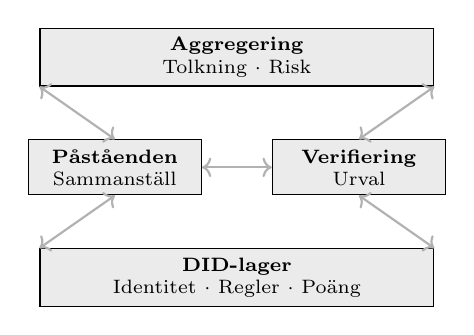
\begin{tikzpicture}[
    layer/.style={draw, minimum height=0.7cm, align=center, font=\scriptsize, fill=black!8},
    arr/.style={<->, thick, gray!60}
]
\node[layer, minimum width=5cm] (agg) at (0,2.8) {\textbf{Aggregering}\\Tolkning\ $\cdot$ Risk};
\node[layer, minimum width=2.2cm] (claim) at (-1.55,1.4) {\textbf{Påståenden}\\Sammanställ};
\node[layer, minimum width=2.2cm] (verif) at (1.55,1.4) {\textbf{Verifiering}\\Urval};
\node[layer, minimum width=5cm] (did) at (0,0) {\textbf{DID-lager}\\Identitet $\cdot$ Regler $\cdot$ Poäng};

\draw[arr] (agg.south west) -- (claim.north);
\draw[arr] (agg.south east) -- (verif.north);
\draw[arr] (claim.east) -- (verif.west);
\draw[arr] (claim.south) -- (did.north west);
\draw[arr] (verif.south) -- (did.north east);
\end{tikzpicture}
\caption{RSN:s fyrlagersarkitektur.}
\label{fig:architecture}
\end{figure}

\subsection{Deltagarroller}

En verifieringstransaktion involverar upp till sex distinkta DID-roller (Fig.~\ref{fig:roles}): \textbf{Utfärdare} ($DID_I$, skapar och lämnar in påståendet), \textbf{Subjekt} ($DID_S$, den DID som påståendet handlar om---kan sammanfalla med Utfärdaren), \textbf{Auktoritet} ($DID_A$, godkänner påståendet mot en avgift; kan även erbjuda vittnestjänster---\emph{valfritt}), \textbf{Vittne} ($DID_{W_{1..n}}$, inkognitoövervakare av verifierarens ärlighet via utmaningskoder---\emph{valfritt}), \textbf{Verifierare} ($DID_V$, algoritmiskt vald att publicera påståendet), och \textbf{RSN} (nätverket där verifierade påståenden publiceras). Vilken roll som helst kan delegeras till en annan DID (Avsnitt~7.4). En Auktoritet paketerar vanligtvis godkännande med vittnestjänster, men de två funktionerna är logiskt oberoende.

\begin{figure}[ht]
\centering
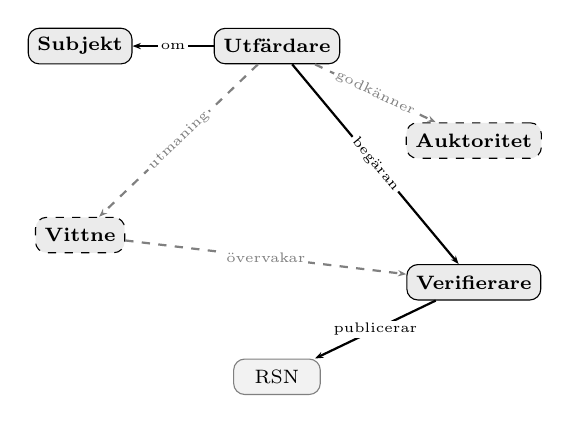
\begin{tikzpicture}[
    role/.style={draw, rounded corners, minimum width=1.1cm, minimum height=0.45cm, align=center, font=\scriptsize, fill=black!8},
    opt/.style={draw, rounded corners, minimum width=1.1cm, minimum height=0.45cm, align=center, font=\scriptsize, fill=black!8, dashed},
    arr/.style={-{Stealth[length=3pt]}, thick},
    oarr/.style={-{Stealth[length=3pt]}, thick, dashed, gray},
    lbl/.style={font=\tiny, fill=white, inner sep=1pt}
]
\node[role] (I) at (0,2.4) {\textbf{Utfärdare}};
\node[role] (S) at (-2.5,2.4) {\textbf{Subjekt}};
\node[opt] (A) at (2.5,1.2) {\textbf{Auktoritet}};
\node[opt] (W) at (-2.5,0) {\textbf{Vittne}};
\node[role] (V) at (2.5,-0.6) {\textbf{Verifierare}};
\node[role, fill=black!5, draw=gray] (N) at (0,-1.8) {RSN};

\draw[arr] (I) -- node[lbl] {om} (S);
\draw[oarr] (I) -- node[lbl,sloped] {godkänner} (A);
\draw[oarr] (I) -- node[lbl,sloped] {utmaning} (W);
\draw[arr] (I) -- node[lbl,sloped] {begäran} (V);
\draw[oarr] (W) -- node[lbl] {övervakar} (V);
\draw[arr] (V) -- node[lbl] {publicerar} (N);
\end{tikzpicture}
\caption{DID-roller i en verifieringstransaktion. Streckad = valfri (Auktoritet, Vittne).}
\label{fig:roles}
\end{figure}

\subsection{Omutbarhet: fyra krafter}

RSN:s omutbarhet uppstår inte ur en enda mekanism utan ur fyra samtidiga krafter. Ingen är tillräcklig ensam; endast deras kombination gör ett korruptionsförsök ekonomiskt irrationellt.

\textbf{Oförutsägbart mål.} Verifieraren för varje påstående väljs ickedeterministiskt genom konsekvent hashning (Avsnitt~5.3). En angripare kan inte i förväg rikta in sig på en specifik verifierare för mutor, eftersom verifierarens identitet är en funktion av påståendets innehåll och tidigare iterationer, inte av utfärdarens val.

\textbf{Ryktesmässig hävstång---långsamt upp, snabbt ner.} Rykte kan endast förvärvas stegvis, genom ihållande konsekvent beteende. Det kan dock förloras katastrofalt genom ett enda bedrägligt godkännande (Avsnitt~6.2). Denna asymmetri innebär att år av ackumulerat rykte kan förstöras av ett oärligt godkännande; den optimala strategin förblir att avvisa misstänkta påståenden.

\textbf{Offentligt löfte.} Varje DID-innehavare deklarerar offentligt sin policy---en maskinläsbar uppsättning regler som de förbinder sig att följa. Avvikelse mellan deklarationen och faktiskt beteende är upptäckbar och prissätts som en ryktesförseelse allvarligare än den underliggande överträdelsen (Avsnitt~7.3). Hyckleri är därför dyrare än direkt oärlighet.

\textbf{Mesh-nätverkets asymmetriska angreppskostnad.} Kostnaden för att censurera eller destabilisera nätverket växer icke-linjärt med nätverkets storlek och täthet, medan kostnaden för att tolerera det förblir konstant. För att censur ska löna sig skulle en centraliserad aktör behöva tillämpa den över hela nätverket---vilket kräver åtgärder oproportionerliga mot någon tänkbar nytta (Avsnitt~10).

% ============================================================
% 4. DECENTRALIZED IDENTITY MODEL
% ============================================================
\section{Modell för decentraliserad identitet}

\subsection{DID med särskilda egenskaper}

RSN utvidgar W3C:s DID Core-specifikation~\cite{did2022} med: \textbf{Deklarerade regler} (maskinläsbara beteendeåtaganden), \textbf{Ryktesmetadata} (aggregerad beteendepoäng), och \textbf{Nätverksdirigering} (föränderlig onion-gateway skild från den stabila ringpositionen).

\subsection{Påståendets livscykel}

Ett påstående fortskrider genom sex steg (Fig.~\ref{fig:lifecycle}): sammanställning, valfritt auktoritetsgodkännande, val av verifierare via konsekvent hashning, verifieringsbeslut (godkänn eller avvisa med iteration), publicering, och ryktesuppdatering för alla parter.

\begin{figure}[ht]
\centering
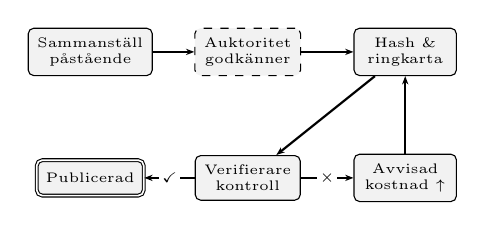
\begin{tikzpicture}[
    stp/.style={draw, rounded corners=2pt, minimum width=1.3cm, minimum height=0.45cm, align=center, font=\tiny, fill=black!5},
    arr/.style={-{Stealth[length=3pt]}, thick},
    lbl/.style={font=\tiny, fill=white, inner sep=1pt}
]
\node[stp] (comp) at (0,0) {Sammanställ\\påstående};
\node[stp, dashed] (auth) at (2.0,0) {Auktoritet\\godkänner};
\node[stp] (hash) at (4.0,0) {Hash \&\\ringkarta};
\node[stp] (ver) at (2.0,-1.6) {Verifierare\\kontroll};
\node[stp, double] (pub) at (0,-1.6) {Publicerad};
\node[stp] (rej) at (4.0,-1.6) {Avvisad\\kostnad $\uparrow$};

\draw[arr] (comp) -- (auth);
\draw[arr] (auth) -- (hash);
\draw[arr] (hash) -- (ver);
\draw[arr] (ver) -- node[lbl] {\checkmark} (pub);
\draw[arr] (ver) -- node[lbl] {$\times$} (rej);
\draw[arr] (rej) -- ++(0,0.8) -| (hash);
\end{tikzpicture}
\caption{Påståendets livscykel med iterationsslinga.}
\label{fig:lifecycle}
\end{figure}

\subsection{Förhållande till W3C DID Core}

RSN:s identitetsmodell är en äkta övermängd av W3C:s DID Core-specifikation~\cite{did2022}. Alla RSN-DID:er är giltiga W3C-DID:er. De RSN-specifika utvidgningarna kodas som egenskaper i DID-dokumentet, definierade i en särskild DID-metodspecifikation, kompatibel med befintlig infrastruktur såsom ION~\cite{buchner2021} och Ceramic~\cite{ceramic2023}.

% ============================================================
% 5. VERIFICATION AND PROPAGATION
% ============================================================
\section{Informationsverifiering och spridning}

\subsection{Kostnaden för informationsinträde}

RSN:s centrala ekonomiska princip är asymmetrin mellan läsning och skrivande. Läsning av ryktesdata närmar sig noll marginalkostnad för deltagare som är del av DID-nätverket och har tillgång i nivå med sitt rykte---nykomlingar måste gradvis förtjäna bredare tillgång (se anti-snyltning). Skrivande---förstått som den varaktiga materialiseringen av rykte in i nätverket, inte som en engångsteknisk handling---kräver verifierbar kumulativ investering över tre dimensioner: \textbf{tid} (levnadsår ägnade åt konsekvent beteende, uppfyllda åtaganden och odlade relationer), \textbf{energi} (ansträngning nedlagd på ärlig handel, omsorg om partnerskap och långsiktig pålitlighet), och \textbf{pengar} (investering i det egna namnet---yrkesutveckling, kvaliteten på det egna arbetet, gottgörelse för orsakad skada). Rykte kan inte köpas omedelbart---det är resultatet av livslång ackumulering som systemet enbart gör synlig och överförbar mellan sammanhang. Protokollets engångstekniska kostnader (kryptografiska signaturer, verifieraravgifter) är försumbara jämfört med denna underliggande investering.

\subsection{Social graf och kontaktdjup}

RSN är i grunden ett socialt nätverk: varje DID lägger till kontakter (andra DID:er) som tillåter kopplingen. Dessa kontakter har sina egna kontakter, och så vidare. Den algoritmiska verifierarsökningen verkar inom ett konfigurerbart djup $h$ av länkade kontakter (t.ex. $h=3$: ens direkta kontakter, deras kontakter, och kontakternas kontakter). Denna arkitektur kräver inte en enda global blockkedja---den gynnar naturligt uppkomsten av gemenskaper/kluster med överlappningar in i andra gemenskaper. Varje DID-deltagare måste ha en publicerad \textbf{policy}---en maskinläsbar uppsättning regler som styr hur inkommande förfrågningar bedöms. Policyöverträdelser registreras i nätverket som negativa artefakter.

\subsection{Algoritmiskt val av verifierare}

Verifieringsprotokollet använder konsekvent hashning~\cite{karger1997} (Fig.~\ref{fig:verifier}). Verifiering är en betald tjänst: verifierare arbetar mot en avgift, vilket skapar en marknad där konkurrens driver prissättning, hastighet och tillförlitlighet.

\textbf{Steg 1.} Påståendedokumentet sammanfogas med föregående iterations hashresultat (eller $\varnothing$ vid första iterationen) och hashas:
\begin{equation}
\text{pos} = f_h(\text{claim} \| \text{prev\_hash})
\label{eq:hash}
\end{equation}

Algoritmen måste inkludera den \emph{fullständiga vägen} av alla tidigare förfrågningar och svar---inte enbart en hash av föregående iteration. Varje verifierares fullständiga svar (godkännande, avslag, offererat pris, skäl) läggs till det växande dokumentet, verifierbart genom kryptografiska signaturer vid varje steg.

\textbf{Steg 2.} Hashen mappas till $N$ positioner på den konsekventa hashringen, jämnt fördelade (t.ex. för $N=4$: $+0^{\circ}, +90^{\circ}, +180^{\circ}, +270^{\circ}$). Från varje position väljer en medurs sökning den närmaste DID:en som verifierarkandidat (Fig.~\ref{fig:multipoint}). $N$ är en variabel parameter som kan bero på andelen för närvarande aktiva DID:er, tid på dygnet, eller nätverkets historiska svarsförmåga.

\textbf{Steg 3.} Verifieraren godkänner (publicerar, satsar rykte) eller avvisar (återgår till Steg~1 med avslagshashen). När en nod inte svarar trots att den deklarerar online-status måste nästa förfrågan inkludera alla svar från alla $N$ tidigare verifierarkandidater.

\textbf{Anti-snyltning.} Mål-DID:er kan sätta avgifter eller åtkomstbegränsningar för förfrågningar från nya DID:er med litet rykte. Denna graderade mekanism (inte binär) tvingar nykomlingar att bygga rykte genom genuin aktivitet innan de fritt konsumerar andras data.

\begin{figure}[ht]
\centering
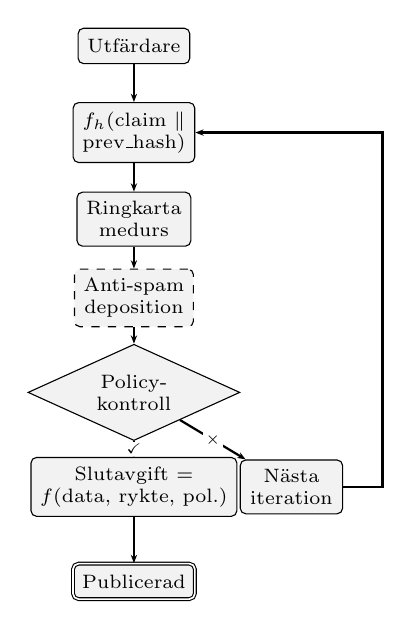
\begin{tikzpicture}[
    box/.style={draw, rounded corners=2pt, minimum width=1.3cm, minimum height=0.45cm, align=center, font=\scriptsize, fill=black!5},
    dec/.style={draw, diamond, aspect=2.2, minimum width=0.9cm, align=center, font=\scriptsize, fill=black!5},
    arr/.style={-{Stealth[length=3pt]}, thick},
    lbl/.style={font=\tiny, fill=white, inner sep=1pt}
]
\node[box] (iss) at (0,0) {Utfärdare};
\node[box] (hash) at (0,-1.1) {$f_h$(claim $\|$\\prev\_hash)};
\node[box] (ring) at (0,-2.2) {Ringkarta\\medurs};
\node[box, dashed] (spam) at (0,-3.2) {Anti-spam\\deposition};
\node[dec] (check) at (0,-4.4) {Policy-\\kontroll};
\node[box] (rej) at (2,-5.6) {Nästa\\iteration};
\node[box] (fee) at (0,-5.6) {Slutavgift =\\$f$(data, rykte, pol.)};
\node[box, double] (pub) at (0,-6.8) {Publicerad};

\draw[arr] (iss) -- (hash);
\draw[arr] (hash) -- (ring);
\draw[arr] (ring) -- (spam);
\draw[arr] (spam) -- (check);
\draw[arr] (check) -- node[lbl] {$\times$} (rej);
\draw[arr] (check) -- node[lbl] {\checkmark} (fee);
\draw[arr] (fee) -- (pub);
\draw[arr] (rej.east) -- ++(0.5,0) |- (hash.east);
\end{tikzpicture}
\caption{Protokoll för val av verifierare. Anti-spam-depositionen är valfri och kan vara återbetalbar. Slutavgiften betalas endast vid godkännande.}
\label{fig:verifier}
\end{figure}

Varje avslag lägger till verifierarens fullständiga svar (inklusive skäl och villkor) till påståendedokumentet, vilket utökar dess innehåll. Från det utökade dokumentet beräknas ickedeterministiskt en ny hash, som mappas till en annan ringposition och väljer en annan verifierare. Dokumentation av hela vägen är obligatorisk---utfärdaren kan inte förutsäga eller påverka nästa verifierare. Om en verifierare ignorerar en förfrågan trots en förenlig deklarerad policy registrerar vittnen (om de finns) detta, och utfärdaren kan bifoga vittnesbevis vid slutpublicering.

\begin{figure}[ht]
\centering
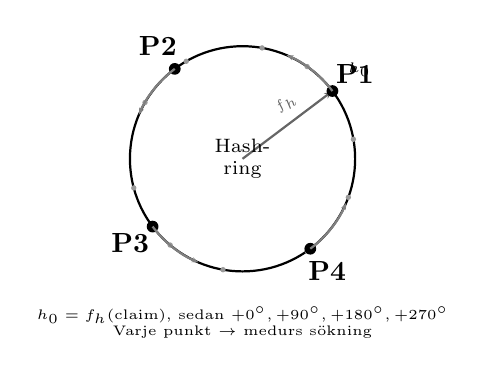
\begin{tikzpicture}[scale=0.65]
% Ring
\draw[thick] (0,0) circle (2.2cm);
% DID nodes on ring
\foreach \a in {10,55,80,120,150,195,230,260,305,340} {
  \fill[black!40] (\a:2.2) circle (1.5pt);
}
% Hash offset arrow pointing to initial position
\draw[-{Stealth[length=3pt]}, thick, black!60] (0,0) -- node[font=\tiny,above,sloped,pos=0.6] {$f_h$} (37:2.2);
\fill[black] (37:2.2) circle (2pt);
\node[font=\tiny,anchor=south west] at (37:2.35) {$h_0$};
% N=4 points offset from h0 by +0, +90, +180, +270
\foreach \offset/\l in {0/P1,90/P2,180/P3,270/P4} {
  \pgfmathsetmacro{\ang}{37+\offset}
  \node[fill=black, circle, inner sep=1.5pt] (p\offset) at (\ang:2.2) {};
  \node[font=\tiny,font=\bfseries] at (\ang:2.75) {\l};
  % clockwise search arc
  \draw[-{Stealth[length=2.5pt]}, thick, gray] (\ang:2.2) arc (\ang:\ang+30:2.2);
}
\node[font=\scriptsize, align=center] at (0,0) {Hash-\\ring};
\node[font=\tiny, align=center] at (0,-3.2) {$h_0 = f_h(\text{claim})$, sedan $+0^{\circ},+90^{\circ},+180^{\circ},+270^{\circ}$\\Varje punkt $\rightarrow$ medurs sökning};
\end{tikzpicture}
\caption{Flerpunktsval ($N{=}4$). Hashen $h_0$ sätter förskjutningen; 4 punkter jämnt fördelade från $h_0$.}
\label{fig:multipoint}
\end{figure}

\subsection{Vittnesprotokoll}

\textbf{Vittnes}-rollen ger inkognito-ansvarsutkrävande för verifierarens ärlighet genom ett kryptografiskt utmaningskodsprotokoll:

\textbf{Steg W1.} Den begärande signerar verifieringsförfrågan och skickar den till $N_w$ vittnen---kontakter från den begärandes sociala nätverk, eller specialiserade leverantörer av vittnestjänster som verkar mot en avgift.

\textbf{Steg W2.} Varje vittne $w_i$ signerar hela den signerade förfrågan, behåller originalsignaturen $\sigma_i$, och beräknar en utmaningskod $c_i = h(\sigma_i)$. Utmaningskoden läggs till förfrågan.

\textbf{Steg W3.} Förfrågan, som nu bär $N_w$ utmaningskoder, skickas till verifieraren. Verifieraren observerar koderna men \emph{kan inte avgöra} vilka vittnena är eller huruvida koderna motsvarar verkliga signaturer.

\textbf{Steg W4 (ärlig verifierare).} Om verifieraren svarar i enlighet med sin deklarerade policy förblir utmaningskoderna ogenomskinliga. Vittnen avslöjas aldrig. Ingen ytterligare data publiceras.

\textbf{Steg W5 (policyöverträdelse).} Om verifieraren bryter mot sin policy (ignorerar förfrågan, svarar inkonsekvent) innehar den begärande vittnenas originalsignaturer $\sigma_i$. Dessa kan publiceras som kompletterande data: vem som helst kan verifiera $c_i = h(\sigma_i)$, vilket bevisar att vittnet var närvarande. Den begärande kan publicera oberoende---verifieraren signerade redan utmaningskoderna i sitt svar.

\textbf{Bluffegenskapen.} Den begärande kan ersätta några eller alla utmaningskoder med slumpmässiga värden. Verifieraren kan inte skilja äkta koder (uppbackade av högt renommerade auktoriteter) från brus. Denna \emph{osäkerhet} är verkställighetsmekanismen: varje förfrågan bär risken att en respekterad auktoritet iakttar inkognito. Kostnaden för att upprätthålla detta tryck är nära noll (att generera slumptal), medan den potentiella kostnaden av oärlighet för verifieraren är katastrofal. Ärligt beteende incitamenteras även i frånvaro av faktiska vittnen.

\textbf{Auktoritet som vittne.} En Auktoritet som godkänner ett påstående kan paketera vittnestjänster: ``Jag godkänner ditt påstående och tjänar som inkognitovittne under verifieringen.'' Detta är en naturlig affärsmodell---Auktoriteten har redan sammanhanget. De två rollerna är dock logiskt oberoende.

\subsection{Principen om dyr radikalism}

Tre kostnadskanaler samverkar samtidigt (Fig.~\ref{fig:radicalism}):

\textbf{Kanal 1: Iterationskostnad.} Varje avslag framtvingar en ny iteration som förbrukar tid och resurser. Linjär tillväxt.

\textbf{Kanal 2: Dokumentuppsvällning.} Varje iteration lägger till verifierarens fullständiga svar till påståendedokumentet. Tillväxten är linjär, men med en basförskjutning: den initiala nyttolasten (påståendets innehåll, auktoritetsgodkännande, kryptografiska signaturer) har redan en icke-trivial storlek $B_0$. Total storlek efter $k$ iterationer: $S(k) = B_0 + k \cdot \Delta$, där $\Delta$ är den genomsnittliga svarsstorleken.

\textbf{Kanal 3: Verifierarens riskpremie.} Risk är subjektiv. Verifieraren bedömer huruvida den begärande DID:ens deklarerade policyer strider mot verifierarens egna kommersiella, sociala eller politiska intressen. Premien kan eskalera exponentiellt med det upplevda avståndet från verifierarens ``ideal'': $P(d) = \alpha \cdot e^{\beta d}$, där $d$ är verifierarens subjektiva avståndsmått. Bortom en personlig no-go-gräns kan verifieraren vägra helt.

\begin{figure}[ht]
\centering
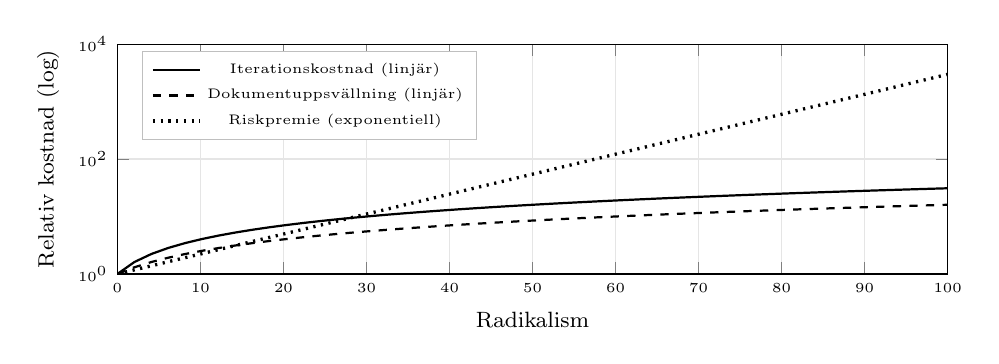
\begin{tikzpicture}
\begin{axis}[
    width=\columnwidth,
    height=4.5cm,
    xlabel={\footnotesize Radikalism},
    ylabel={\footnotesize Relativ kostnad (log)},
    ymode=log,
    xmin=0, xmax=100,
    ymin=1, ymax=10000,
    grid=major,
    grid style={gray!20},
    legend style={at={(0.03,0.97)},anchor=north west,font=\tiny,draw=gray!50},
    tick label style={font=\tiny},
    label style={font=\footnotesize},
]
\addplot[black, thick, domain=0:100, samples=50] {1 + 0.3*x};
\addlegendentry{Iterationskostnad (linjär)}
\addplot[black, thick, dashed, domain=0:100, samples=50] {1 + 0.15*x};
\addlegendentry{Dokumentuppsvällning (linjär)}
\addplot[black, thick, dotted, line width=1.2pt, domain=0:100, samples=100] {exp(0.08*x)};
\addlegendentry{Riskpremie (exponentiell)}
\end{axis}
\end{tikzpicture}
\caption{Kostnadseskalering över tre kanaler. Riskpremien dominerar vid hög radikalism.}
\label{fig:radicalism}
\end{figure}

Avgörande är att detta inte är censur. Inget påstående är förbjudet. Systemet prissätter risk (Tabell~\ref{tab:costs}).

\begin{table}[ht]
\centering
\caption{Kostnadsjämförelse mellan påståendetyper.}
\label{tab:costs}
\footnotesize
\begin{tabular}{@{}lcccc@{}}
\toprule
\textbf{Typ} & \textbf{Iter.} & \textbf{Dok} & \textbf{Avgift} & \textbf{Totalt} \\
\midrule
Trovärdig & $k_{\min}$ & $B_0$ & $P_{\min}$ & Låg \\
Kontroversiell & $k_{\text{med}}$ & $B_0{+}k\Delta$ & $\alpha e^{\beta d}$ & Måttlig \\
Radikal & $k_{\max}$ & $\gg B_0$ & $\gg P_{\min}$ & Mycket hög \\
Bedräglig & $\to\infty$ & --- & --- & Opublicerbar \\
\bottomrule
\end{tabular}
\end{table}

% ============================================================
% 6. REPUTATION AND RISK
% ============================================================
\section{Rykte och riskbedömning}

\subsection{Modell för ryktesackumulering}

Rykte uppvisar tre egenskaper: \textbf{långsam ackumulering} (stegvis tillväxt genom konsekvent beteende), \textbf{snabb förstörelse} (ett enda bedrägeri kan sänka poängen katastrofalt), och \textbf{individuell bedömning} (varje konsumerande part kan tillämpa sin egen aggregeringsfunktion).

\subsection{Renommerade auktoriteter}

En Renommerad Auktoritet granskar påståenden och, om den är tillfredsställd, medsignerar dem---och satsar sitt eget rykte (Fig.~\ref{fig:authority}). Asymmetrin är avsiktlig: att vinna rykte är långsamt (stegvis $+\delta$ per ärligt godkännande), medan att förlora det är katastrofalt ($-\Delta \gg \delta$ per falskt godkännande; illustrativt t.ex. $+2\%$ mot $-70\%$). Den optimala strategin är alltid att avvisa misstänkta påståenden. De specifika värdena på $\delta$ och $\Delta$ är systemparametrar.

\begin{figure}[ht]
\centering
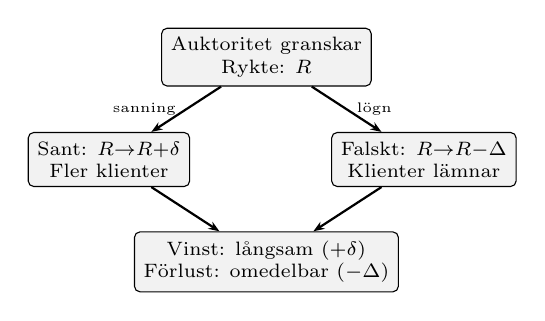
\begin{tikzpicture}[
    box/.style={draw, rounded corners=2pt, minimum width=2cm, minimum height=0.6cm, align=center, font=\scriptsize, fill=black!5},
    arr/.style={-{Stealth[length=4pt]}, thick}
]
\node[box] (exam) at (0,0) {Auktoritet granskar\\Rykte: $R$};
\node[box] (true) at (-2,-1.3) {Sant: $R{\to}R{+}\delta$\\Fler klienter};
\node[box] (false) at (2,-1.3) {Falskt: $R{\to}R{-}\Delta$\\Klienter lämnar};
\node[box] (insight) at (0,-2.6) {Vinst: långsam ($+\delta$)\\Förlust: omedelbar ($-\Delta$)};

\draw[arr] (exam) -- node[left,font=\tiny] {sanning} (true);
\draw[arr] (exam) -- node[right,font=\tiny] {lögn} (false);
\draw[arr] (true) -- (insight);
\draw[arr] (false) -- (insight);
\end{tikzpicture}
\caption{Renommerad Auktoritet---asymmetriska incitament.}
\label{fig:authority}
\end{figure}

\subsection{Flerdimensionellt rykte}

Rykte är inte en skalär utan en vektor över flera dimensioner: finansiell pålitlighet, personlig integritet, yrkeskompetens, samhällsengagemang, med flera (Fig.~\ref{fig:reputation-radar}). Olika bedömningsleverantörer projicerar denna vektor olika beroende på sammanhang---en långivare prioriterar finansiell pålitlighet, en arbetsgivare yrkeskompetens, en granne samhällsbeteende. Det finns ingen enda ``korrekt'' ryktespoäng; endast perspektiv.

\begin{figure}[ht]
\centering
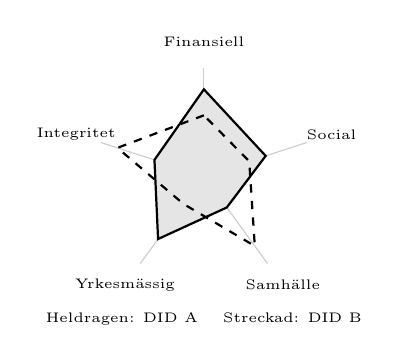
\begin{tikzpicture}[scale=0.55]
\foreach \a/\l in {90/Finansiell,162/Integritet,234/Yrkesmässig,306/Samhälle,18/Social} {
  \draw[gray!40] (0,0) -- (\a:2.5);
  \node[font=\tiny, align=center] at (\a:3.1) {\l};
  \foreach \r in {0.8,1.6,2.4} {
    \fill[black!15] (\a:\r) circle (0.5pt);
  }
}
\draw[thick, fill=black!10] (90:2.0) -- (162:1.2) -- (234:1.8) -- (306:0.9) -- (18:1.5) -- cycle;
\draw[thick, dashed] (90:1.4) -- (162:2.1) -- (234:0.8) -- (306:2.0) -- (18:1.1) -- cycle;
\node[font=\tiny] at (0,-3.3) {Heldragen: DID A \quad Streckad: DID B};
\end{tikzpicture}
\caption{Flerdimensionella ryktesvektorer. Olika DID:er uppvisar olika profiler över dimensioner.}
\label{fig:reputation-radar}
\end{figure}

\subsection{Demokratiserad riskbedömning}

RSN demokratiserar systematisk riskbedömning---en förmåga som för närvarande är koncentrerad till finansinstitut men tillämpbar långt bortom bankväsendet. Industrikonglomerat som bedömer leverantörers tillförlitlighet, försäkringsbolag som prissätter beteenderisk, due diligence vid fusioner och förvärv, uppskattning av utrustnings livslängd inom tillverkning---överallt där motpartsrisk kräver bedömning tillhandahåller RSN ett decentraliserat, marknadsdrivet alternativ. En marknad av tolkningstjänster översätter rå flerdimensionell ryktesdata till användbara sammanfattningar, vilket gör motpartsbedömning tillgänglig för varje deltagare till marginalkostnad.

% ============================================================
% 7. CONSENSUS AND DISPUTE RESOLUTION
% ============================================================
\section{Konsensus och tvistlösning}

\subsection{Modell för decentraliserad rättvisa}

RSN omformulerar rättvisa som ett bilateralt förhandlingsproblem. Hotet om permanent, verifierbar ryktesskada är ett effektivare avskräckningsmedel än rättsprocesser som den skadade parten inte har råd med.

\subsection{Emergent konsensus}

Varje deltagare upprätthåller en personlig tillfredsställelsetröskel. Nätverkets aggregerade konsensus uppstår som det statistiska genomsnittet av tusentals bilaterala förhandlingar (Fig.~\ref{fig:consensus}). Ett svar långt över konsensus (barbariskt) är dyrt att publicera. Ett svar nära konsensus (proportionellt) är billigt. Konsensus är inte en regel---det är en prissignal.

\begin{figure}[ht]
\centering
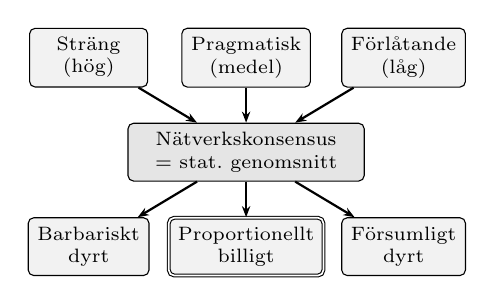
\begin{tikzpicture}[
    person/.style={draw, rounded corners=2pt, minimum width=1.5cm, minimum height=0.5cm, align=center, font=\scriptsize, fill=black!5},
    arr/.style={-{Stealth[length=4pt]}, thick}
]
\node[person] (a) at (-2,0) {Sträng\\(hög)};
\node[person] (b) at (0,0) {Pragmatisk\\(medel)};
\node[person] (c) at (2,0) {Förlåtande\\(låg)};
\node[person, fill=black!10, minimum width=3cm] (cons) at (0,-1.2) {Nätverkskonsensus\\= stat.\ genomsnitt};
\node[person] (exp) at (-2,-2.4) {Barbariskt\\dyrt};
\node[person, double] (prop) at (0,-2.4) {Proportionellt\\billigt};
\node[person] (neg) at (2,-2.4) {Försumligt\\dyrt};

\draw[arr] (a) -- (cons);
\draw[arr] (b) -- (cons);
\draw[arr] (c) -- (cons);
\draw[arr] (cons) -- (exp);
\draw[arr] (cons) -- (prop);
\draw[arr] (cons) -- (neg);
\end{tikzpicture}
\caption{Emergent konsensus från individuella tillfredsställelsetrösklar.}
\label{fig:consensus}
\end{figure}

\subsection{Bestraffningskalibrering}

Varje DID-innehavare deklarerar offentligt svar på specifika kategorier av missförhållanden. Oproportionerligt hårda eller milda deklarationer drar till sig negativa ryktessignaler. Proportionella deklarationer accepteras utan friktion---ett självkalibrerande bestraffningssystem.

Konsensusdeklarationer är själva föremål för hyckleridetektering: att deklarativt förbinda sig till en konsensusposition medan man beter sig inkonsekvent utgör en ryktesförseelse allvarligare än den underliggande avvikelsen, eftersom den påvisar avsiktligt bedrägeri.

\subsection{Delegering}

Alla aktiviteter inom en DID---med ett undantag---kan delegeras till en annan DID. \textbf{Subjektsrollen---den DID vars beteende påståendet handlar om---kan inte delegeras; den är icke-överförbart bunden till den identitetsinnehavare som påståendet refererar till.} De övriga aktiva rollerna---Utfärdare, Auktoritet, Vittne, Verifierare---kan överföras till en utsedd delegat-DID, vare sig för verifiering, inlämning av påståenden, konsensusdeltagande eller tvistlösning. Delegering är återkallelig när som helst. Detta möjliggör specialisering (t.ex. professionella verifieringstjänster) medan Innehavaren behåller den yttersta kontrollen och ansvaret. Delegering gäller över hela systemet och är väsentlig för skalbarhet.

\subsection{Från individuell moral till emergent samhällskontrakt}

Varje DID:s deklarerade policy representerar en formalisering av individuell moral: vad Innehavaren anser acceptabelt, hur de svarar på specifika beteenden, vad de kräver av motparter. Dessa policyer påtvingas inte av en systemdesigner---de väljs av varje deltagare och uttrycks i maskinläsbar form.

Denna formalisering möjliggör en emergens i tre steg. Först kodas individuell moral som \textbf{policy}---en uppsättning deklarerade regler, trösklar och svarsfunktioner som DID:en förbinder sig att följa. För det andra producerar summan av alla policyer över nätverket \textbf{emergent etik}---statistiskt observerbara normer som ingen enskild deltagare utformat men som uppstår ur interaktionen mellan tusentals individuella moraliska ståndpunkter~\cite{durkheim1893}. För det tredje utgör denna emergenta etik, uttryckt som delade beteendenormer som upprätthålls genom bilaterala prissignaler, ett \textbf{mätbart samhällskontrakt}---inte en teoretisk konstruktion som ingen undertecknat~\cite{rawls1971}, utan en empiriskt observerbar uppsättning regler uppbackad av faktiskt beteende.

Denna process speglar rön från teorin om moraliska grunder~\cite{haidt2012}: mänsklig moral är intuitiv, pluralistisk och kulturellt variabel. RSN kräver inte moralisk konsensus som indata; den producerar beteendekonsensus som utdata. Det resulterande samhällskontraktet är inte statiskt---det utvecklas allteftersom deltagare ansluter sig, lämnar och justerar sina policyer som svar på nätverksåterkoppling. Till skillnad från klassisk samhällskontraktsteori är detta kontrakt återkalleligt, observerbart och verkställbart utan en suverän.

% ============================================================
% 8. ECONOMIC MODEL
% ============================================================
\section{Ekonomisk modell}

De föregående avsnitten beskrev ett verktyg---RSN:s verifieringsmekanismer, kostnadsstruktur och emergenta konsensus. Detta avsnitt beskriver en metodik för att tillämpa detta verktyg på fiskal och styrningsmässig övergång. Verktyget är allmängiltigt; metodiken nedan är en möjlig tillämpning.

\subsection{Incitamentsstruktur}

Rykte som kapital skapar direkta incitament för ärligt beteende. Vid normal drift bygger deltagare rykte naturligt genom vardagliga transaktioner och uppfyllda åtaganden. Den primära utgiften är på \emph{negativa} påståenden---att registrera skada orsakad av andra. Denna asymmetri incitamenterar nyttigt, tillförlitligt beteende: att vara ärlig kostar inget extra, medan att vara skadlig skapar ett dokumenterat spår som andra kommer att betala för att bevara. Hyckleri---att deklarera regler utan att följa dem---är det dyraste felläget, eftersom det påvisar avsiktligt bedrägeri.

\subsection{Parallellt fiskalt system}

Tre komponenter möjliggör konkurrenstryck: (1)~\textbf{Enkel skatt}---en enda proportionell sats utan undantag, inledningsvis marginellt under den befintliga effektiva satsen; (2)~\textbf{Elektronisk utgiftsregistrering (ESR)}---som inverterar den tjeckiska EET-modellen så att medborgarna övervakar statliga utgifter; (3)~\textbf{Medborgarstyrd skatteallokering}---som börjar på några få procent första året och når, efter ett decennium, allt från låga tvåsiffriga tal till en fullständig migration till ett medborgarstyrt system, beroende på införandetakten. Den faktiska takten beror på hur snabbt fri marknads alternativ till statliga tjänster uppstår och på statens vilja att samarbeta med övergången; tidsfunktionen behöver inte vara linjär, och det finns ingen anledning att sätta en övre gräns för var införandet slutligen kan hamna.

% ============================================================
% 9. MIGRATION PATH
% ============================================================
\section{Migrationsväg}

Migrationen fortskrider genom tre faser (Fig.~\ref{fig:migration}): \textbf{Fas~1: Överlagring} (RSN som informationslager, staten är enda leverantör), \textbf{Fas~2: Konkurrens} (RSN tillhandahåller funktionella alternativ, användning av dubbla system), och \textbf{Fas~3: Övergång} (RSN överträffar statliga motsvarigheter, frivillig migration). Övergången är reversibel i varje skede.

\begin{figure}[ht]
\centering
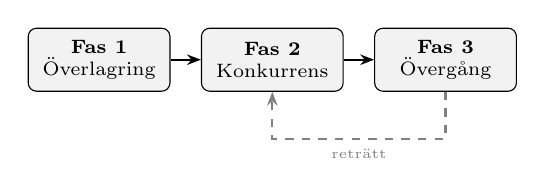
\begin{tikzpicture}[
    phase/.style={draw, rounded corners=3pt, minimum width=1.8cm, minimum height=0.8cm, align=center, font=\scriptsize, fill=black!5},
    arr/.style={-{Stealth[length=5pt]}, thick}
]
\node[phase] (p1) at (0,0) {\textbf{Fas 1}\\Överlagring};
\node[phase] (p2) at (2.2,0) {\textbf{Fas 2}\\Konkurrens};
\node[phase] (p3) at (4.4,0) {\textbf{Fas 3}\\Övergång};

\draw[arr] (p1) -- (p2);
\draw[arr] (p2) -- (p3);
\draw[arr, dashed, gray] (p3.south) -- ++(0,-0.6) -| node[below,font=\tiny,pos=0.25] {reträtt} (p2.south);
\end{tikzpicture}
\caption{Migration i tre faser---reversibel i varje skede.}
\label{fig:migration}
\end{figure}

Den primära tryckmekanismen är fiskal: när villkorliga skattebetalare når en ``ekonomiskt betydande minoritet $X$''---en grupp tillräckligt stor för att repression mot den orsakar icke-triviala ekonomiska skador och civil olydnad blir ett trovärdigt hot---inleder staten förhandling. För illustration använder vi $X \approx 15\%$ av BNP, men den faktiska tröskeln beror på den specifika ekonomin.

% ============================================================
% 10. SECURITY ANALYSIS
% ============================================================
\section{Säkerhetsanalys}

Vi betraktar fem kategorier av motståndare: enskilda illasinnade aktörer, organiserade grupper, företagsmotståndare, motståndare på statsnivå, och motståndare på protokollnivå.

\textbf{Sybil-resistens}~\cite{douceur2002}. Att bygga rykte kräver ihållande, verifierbar interaktion. Kostnaden för en framgångsrik Sybil-attack skalar linjärt med falska identiteter och kvadratiskt med målets ryktesnivå. Att driva flera DID:er parallellt är möjligt men dyrt av design---varje identitet måste oberoende ackumulera rykte genom genuin aktivitet. I fria samhällen avskräcker denna kostnad tillfälligt missbruk; i diktaturer blir parallella DID:er ett överlevnadsverktyg som möjliggör uppdelat motstånd, underjordisk samordning och säkrare navigering på svarta marknaden.

\textbf{Försvar mot maskopi.} Mönster av ömsesidigt godkännande bland slutna grupper är upptäckbara genom analys av den sociala grafen. Ryktesaggregeringsfunktioner nedvärderar påståenden från tätt klustrade källor.

\textbf{Motståndare på statsnivå.} Onion-dirigering, avsaknaden av centraliserad infrastruktur, och fördelningen av Verifierarrollen över deltagarbasen säkerställer att undertryckande kräver åtgärder oproportionerliga mot någon nytta.

\textbf{Integritet kontra ansvarsutkrävande.} Pseudonymitet---en medelväg mellan anonymitet och identitetsavslöjande---tillåter DID:er att ackumulera meningsfullt rykte utan att avslöja Innehavarens verkliga identitet.

% ============================================================
% 11. PRIVACY
% ============================================================
\section{Integritetsöverväganden}

RSN:s integritetsmodell är byggd på pseudonymitet. Innehavaren styr identitetsavslöjandet: minimalt (ren pseudonym), selektivt (specifika referenser länkade), eller fullständigt (juridisk identitet associerad). Publicerade påståenden är permanenta---systemet stödjer kontextuell korrigering men inte radering. En Innehavare kan överge en komprometterad DID och börja på nytt, och förverkar då ackumulerat rykte.

% ============================================================
% 12. RELATED WORK
% ============================================================
\section{Relaterat arbete}

W3C:s DID Core-specifikation~\cite{did2022} och Ceramic Network~\cite{ceramic2023} tillhandahåller identitetsgrunden. EigenTrust~\cite{kamvar2003} demonstrerade distribuerad ryktesaggregering utan central auktoritet. SBT:er~\cite{weyl2022} introducerade icke-överförbara sociala token. RSN skiljer sig i sin betoning på ekonomisk kostnad som ett kvalitetsfilter och sin mekanism för att prissätta radikalism.

DAO:er~\cite{buterin2014} och kvadratisk röstning~\cite{buterin2019} demonstrerade genomförbarheten av decentraliserad styrning. RSN härleder konsensus från bilaterala prisförhandlingar snarare än röstning.

Förslaget bygger på anarkokapitalistisk teori~\cite{rothbard1973,hoppe2001} för privat tjänsteleverans men avviker i två avgörande avseenden: det designar för illvilja och hämndlystna impulser snarare än att förutsätta rationalitet, och det föreslår gradvis övergång snarare än revolution. Konceptet emergenta samhällskontrakt har föregångare i Hayeks teori om spontan ordning~\cite{hayek1973}.

\textbf{Anarko-agorism.} RSN delar betydande gemensam grund med agoristisk motekonomi~\cite{konkin2006}---särskilt betoningen på att bygga parallella institutioner och frivilligt utbyte. Agorismen tenderar dock att förutsätta rationellt egenintresse som en tillräcklig samordningsmekanism och saknar ofta en konkret migrationsväg från befintliga statsstrukturer. RSN införlivar uttryckligen icke-rationella beteendeböjelser och tillhandahåller en fiskal tryckmekanism för gradvis övergång.

\textbf{Meritokrati.} RSN kan representera en första funktionell beskrivning av hur meritokrati~\cite{young1958} kan uppstå som en systemisk egenskap snarare än en slogan. Traditionella meritokratiska system misslyckas eftersom de kräver en central auktoritet för att definiera och upprätthålla ``förtjänst''. I RSN uppstår förtjänst ur bilaterala bedömningar: de som levererar värde ackumulerar rykte; ingen kommitté avgör vem som har förtjänst.

\textbf{Egendom som privilegium.} RSN avviker grundläggande från anarkokapitalistiska och österrikiska skolans behandlingar av äganderätt som naturlig och absolut. I RSN-ramverket är egendom ett \emph{privilegium}---ett socialt erkännande som i extrema fall kan dras tillbaka av gemenskapen när en deltagare grundläggande bryter mot delade normer (svek, vägran att försvara gemenskapen i en existentiell kris, systematisk exploatering). Detta är inte statlig expropriation utan ett tillbakadragande av socialt erkännande från nätverket av bilaterala relationer.

% ============================================================
% 13. LIMITATIONS
% ============================================================
\section{Diskussion och begränsningar}

\textbf{Kallstart.} RSN:s värde beror på nätverkseffekter; tidiga användare möter begränsat värde tills deltagandet når en tröskel. Även från tidiga skeden fungerar dock DID-nätverket som en användbar kompletterande informationskälla. Tidig ryktesbedömning och auktoritetsbedömning förväntas utvecklas gradvis med ökande sofistikering.

\textbf{Anti-snyltning och åtkomstkontroll.} Mål-DID:er kan införa graderade avgifter och åtkomstbegränsningar för förfrågningar från DID:er med lågt rykte. Detta är inte binärt utan en kontinuerlig skala: ju mindre rykte en förfrågande DID har, desto mindre information får den, desto längre väntar den, och desto mer betalar den. Denna mekanism incitamenterar genuint deltagande framför passiv konsumtion.

\textbf{Ojämlik tillgång.} Kostnaden för att publicera påståenden kan filtrera bort legitima klagomål från ekonomiskt missgynnade deltagare. Motåtgärd: varje deltagare fungerar samtidigt som en potentiell verifierare (eller delegerar denna roll) och tjänar verifieringsavgifter. Över en tillräcklig tidshorisont bör en icke-radikal deltagare närma sig finansiell neutralitet---verifieringsintäkter som ungefär uppväger publiceringskostnader. Detta är en statistisk förväntan, inte en garanti.

\textbf{Ryktesojämlikhet.} Tidiga användare ackumulerar fördelar som kan skapa hinder för senkomlingar. Ryktesbedömning utförs dock av tredjepartsleverantörer som kan välja att mildra förstahandsfördelen genom sina aggregeringsalgoritmer. Att vara först med ett gott rykte är en legitim komparativ ekonomisk fördel---och det är avsiktligt.

\textbf{Öppna frågor.} Optimala kostnadsfunktioner, aggregeringsstandarder, protokollstyrning, och interaktion med AI-genererad syntetisk ryktesdata förblir områden för framtida arbete.

Denna uppsats hävdar inte att RSN kommer att producera optimala utfall under alla omständigheter. Den hävdar att RSN representerar ett \emph{genomförbart} alternativ---tekniskt implementerbart, ekonomiskt självförsörjande, och socialt förenligt med mänskliga beteendeböjelser som de faktiskt är.

% ============================================================
% 14. CONCLUSION
% ============================================================
\section{Slutsats}

Denna uppsats har presenterat det ryktes-sociala nätverket, ett decentraliserat protokoll som möjliggör pseudonymt, verifierbart ryktesutbyte. Principen om dyr radikalism säkerställer att bedrägliga påståenden prissätts bort utan censur. Den föreslagna migrationsvägen möjliggör en gradvis, reversibel övergång från befintliga institutioner. Designen införlivar den mänskliga naturen som den är---inklusive småaktighet, illvilja och begäret efter hämndlysten tillfredsställelse---snarare än att kräva ideologisk omvandling. Resultatet är inte utopi utan ett system där rättvisa är tillgänglig, rykte förtjänas, och kostnaden för missförhållanden bärs av den part som orsakade dem.

% ============================================================
% REFERENCES
% ============================================================
\bibliography{references}

\end{document}
